To validate our method we will run the alignment approach of task tree generation against the same case study as Harms et al. did.

\begin{itemize}
	
	\item Two case studies: 
		\begin{itemize}
			\item Application portal case study. 
			\item Website of research group
		\end{itemize}
	\item Table of Case studies
	\item Screenshot of Application Master Portal
	\item Screenshot of Website of research group
	\item Show XML recorded traces
	\item When running the full case study alot of perfomance problems came up.
	\item Memory consumption and computation time grew alot due to the nature of the algorithm
	\item Computation moved from a Intel(R) Core(TM) i5-2520M CPU @ 2.50GHz with 8GB Ram to a AMD Opteron(TM) Processor 6276 (64 core) with 250GB Ram.
	\item The java virtual machine was given 64GB
	\item Still computation time extremly large (see performance evaluation)
	\item Maybe change stop criterium: 10% of the matches found in the first run
	\item Other solution: Update substution matrix, so non-Event tasks can have a negative score (less likely to find matches then)
\end{itemize} 

\section{Data Preprocessing}
After loading the xml file the following preprocessing steps have been performed (shortly explain every step with 1 or 2 sentences)
\begin{itemize}
	\item condenseHTMLGUIModel sequences
	\item condenseMouseClicks sequences
	\item correctKeyInteractionTargets sequences
	\item correctTabKeyNavigationOrder sequences
\end{itemize}

\section{Evaluation of termination conditions}
\begin{itemize}
	\item Run CTA with full case study
	\item show matches found per iteration and time per iteration
\end{itemize}


\section{Performance Evaluation}
\begin{itemize}
	\item Compare Core-TaskTrees(CT) with Core-TaskTrees-Algignment (CTA)
	\begin{itemize}
		\item Run CT with 10, 100, 1000, all user sessions on CS1
		\item Run CTA with 10, 100, 1000, all user sessions on CS1
		\item Show percentage of each step of CTA of all user sessions
		\item Run CT with 10, 100, 1000, all user sessions on CS2
		\item Run CTA with 10, 100, 1000, all user sessions on CS2
		\item Show percentage of each step of CTA of all user sessions
	\end{itemize}
	\item Alot of tables (which step of the algorithm takes how long, for each dataset
\end{itemize}

\section{Generated Task Trees}
\begin{itemize}
	\item Show some meaningful generated task trees
	\item Show also tasktrees that are not useful
\begin{figure}
	\centering
	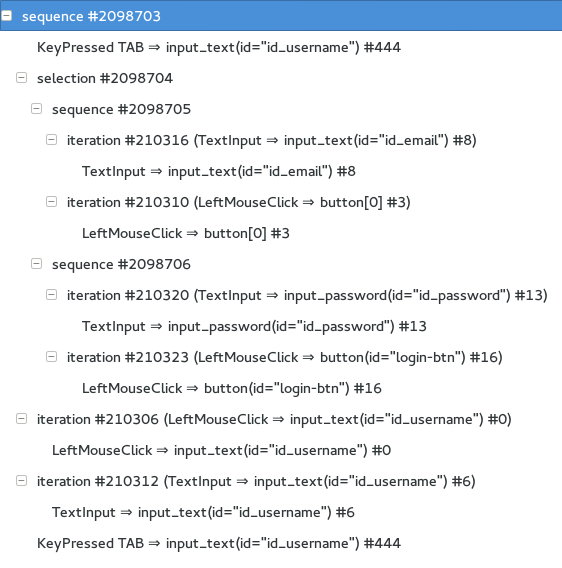
\includegraphics[]{chapters/casestudy/mixedtasktree.png}
	\caption{}
	\label{}
\end{figure}
\begin{figure}
	\centering
	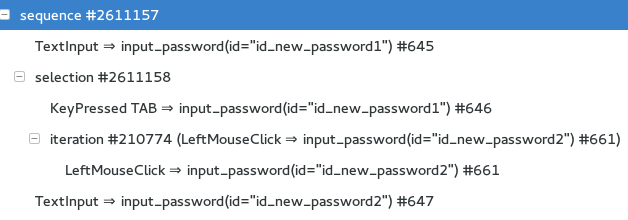
\includegraphics[]{chapters/casestudy/newpassword.png}
	\caption{}
	\label{}
\end{figure}
\begin{figure}
	\centering
	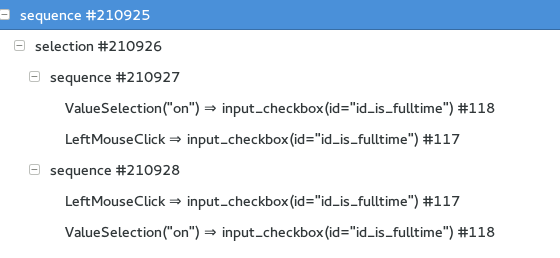
\includegraphics[]{chapters/casestudy/preprocessing_needed.png}
	\caption{}
	\label{}
\end{figure}
\begin{figure}
	\centering
	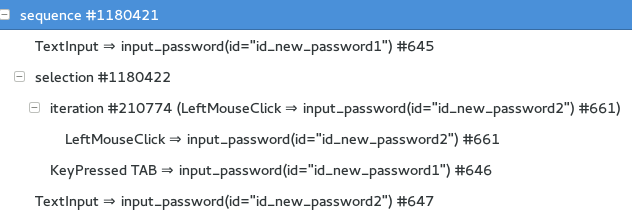
\includegraphics[]{chapters/casestudy/newpassword-1.png}
	\caption{}
	\label{}
\end{figure}
\begin{figure}
	\centering
	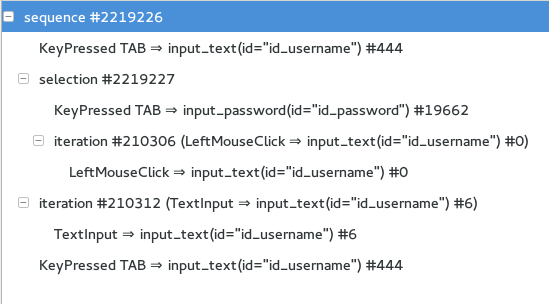
\includegraphics[]{chapters/casestudy/login_process_repeated.png}
	\caption{}
	\label{}
\end{figure}
%\begin{figure}
%	\centering
%	\includegraphics[]{}
%	\caption{}
%	\label{}
%\end{figure}
\end{itemize}


\section{Discussion}
\begin{itemize}
	\item Task Graph
\end{itemize}
